\documentclass[11pt]{amsbook}

\usepackage{../HBSuerDemir}	% ------------------------

\begin{document}

% ++++++++++++++++++++++++++++++++++++++
\hPage{b1p1/271}
% ++++++++++++++++++++++++++++++++++++++
\begin{exmp}
Given the points A(t,3), B(4,5) and C(4,8)
 \begin{hEnumerateAlpha}
    \item Find t if A, B, C are collinear (Points of the same line)
    \item Setting $t=-2$ find the equations of the line AB and BC
    \item Find the equation of the line through B and P(1, -1)
    \item Find $\hDif(P, BC), \hDif(P, AB)$
 \end{hEnumerateAlpha}
 \end{exmp}
\begin{hSolution}
\begin{hEnumerateAlpha}
\item Setting the coordinate of the point in $Ax+ By+ C = 0$   we have the HLS
$$tA + 3B + C = 0$$
$$4A + 5B + C = 0$$
$$4A + 8B + C = 0$$
To have a non trivial solution we get
$$
    \begin{pmatrix} 
    t&3&1  \\
    4&5&1  \\
    4&8&1  
    \end{pmatrix}
    = 0\quad giving\quad t = 4
$$
This is one of the way solution. The others are:
\begin{hEnumerateArabic}
\item By the use of distance: For the collinearity, one of $|AB|, |BC|, |CA|$ must be the sum of the other two.
\item By the use of slope: For the collinearity, the slopes of AB and BC must be equal.
\item By the use of equation: For the collinearity the coordinate of one of the points,say of A, must satisfy the equation of the line through the other two points B, C.(This mean that $d(A, BC)= 0$)
\end{hEnumerateArabic}
\item 
\[
    \begin{split}
    \frac{x-x_1}{x_2-x_1} \quad &\frac{y-y_1}{y_2-y_1}\Longrightarrow \\
    &AB: \frac{x+2}{y+2} \quad \frac{y-3}{y-3} \Longrightarrow \quad x-3y+11=0, \\
    &BC: x_1 = x_2 = 4 \quad \Longrightarrow x = 4
    \end{split}
\]




\end{hEnumerateAlpha}
\end{hSolution}





























% =======================================================
\end{document}  

%==== templates ====

%==== environments ====

%\begin{figure}[htb]
%	\centering
%	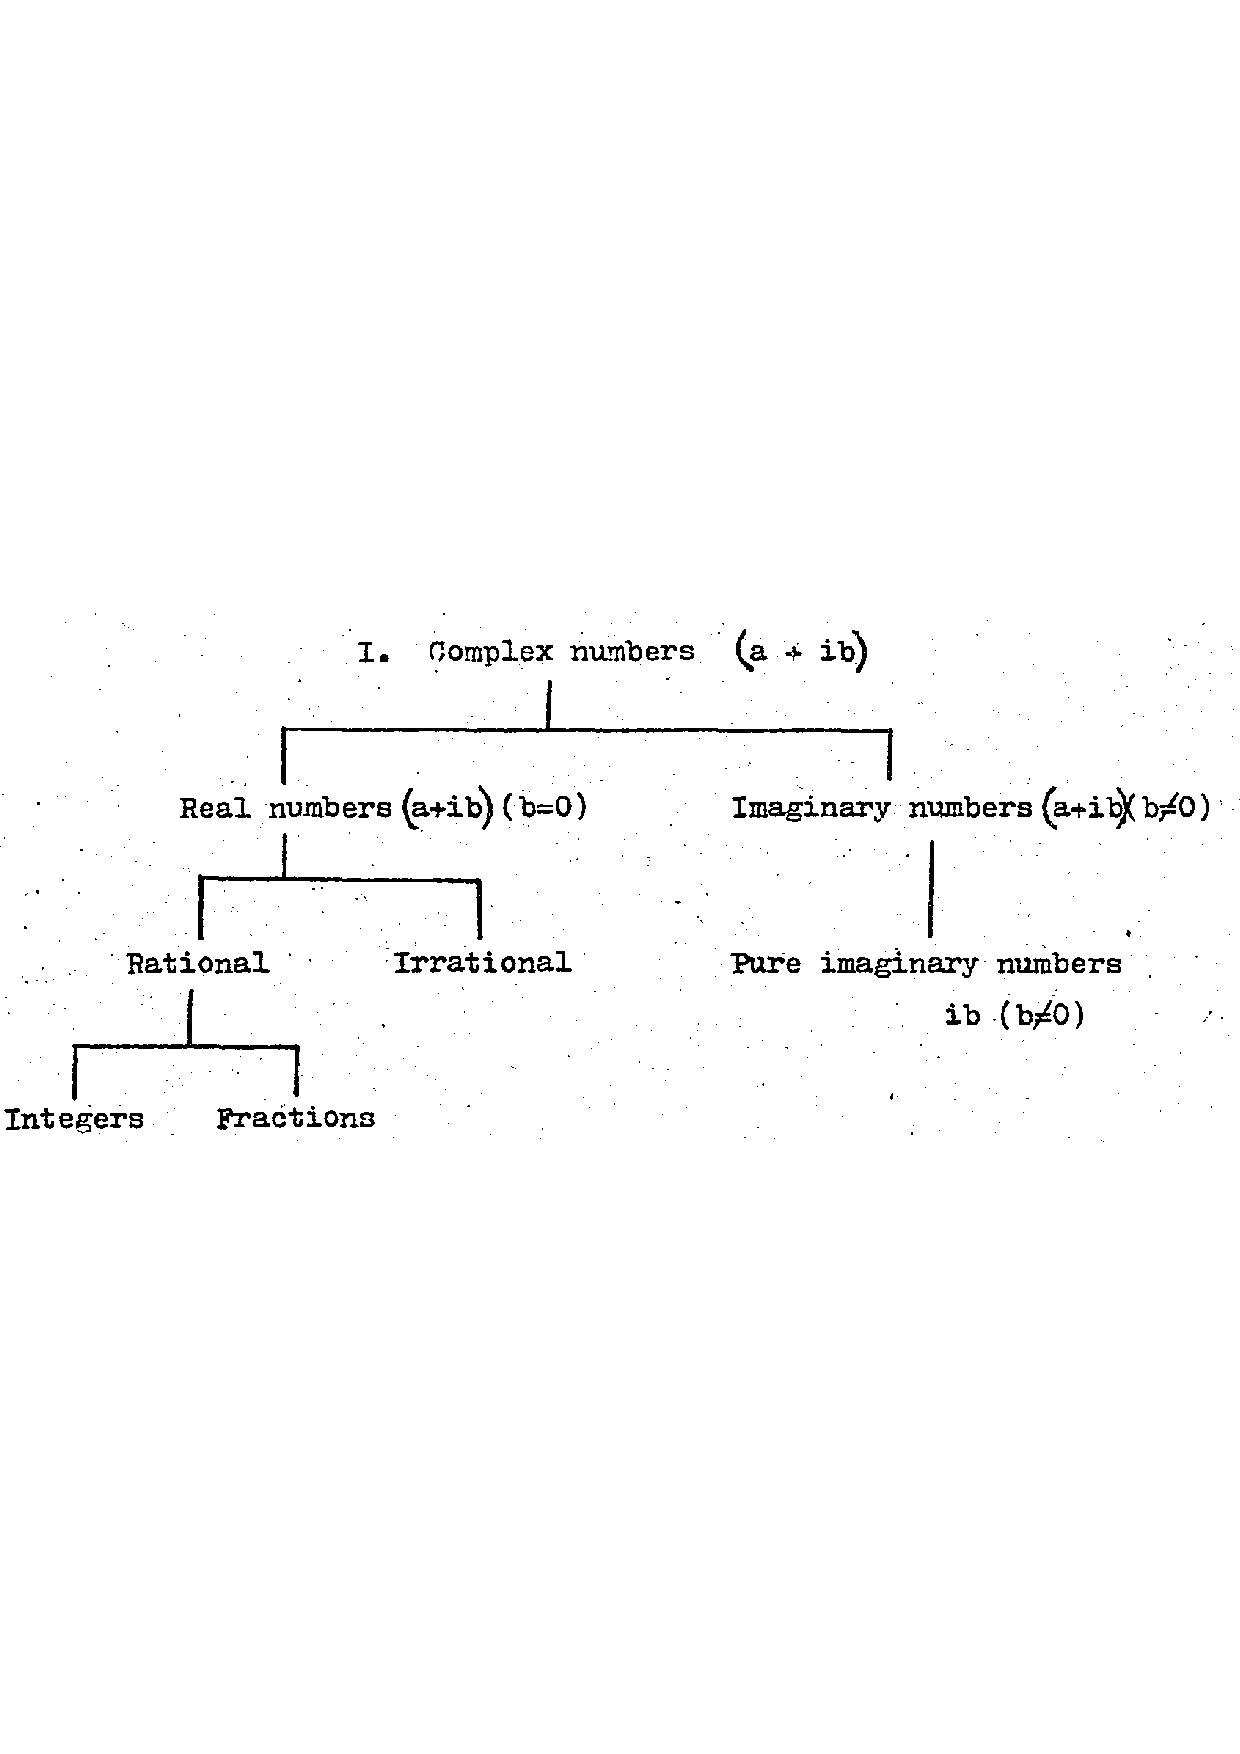
\includegraphics[width=0.9\textwidth]{images/SD-1-1p15A}
%	\caption{Classification of complex numbers}
%	\label{fig:classificationOfComplexNumbersA}
%\end{figure}

%\begin{center}
%\begin{tabular}{cc}
%\end{tabular}
%\end{center}

%\begin{exmp}
%\begin{hSolution}
%\end{hSolution}
%\end{exmp}

%\begin{hEnumerateAlpha}
%\end{hEnumerateAlpha}

%\begin{hEnumerateRoman}
%\end{hEnumerateRoman}

%$
%\begin{bmatrix}
%\end{bmatrix}
%$

%\frac{aaaa}{bbb}
%\frac{a_{n}}{b_{n}}
%\left( aaaa \right)
%\Longrightarrow

%\begin{multicols}{2}
%	bb
%\columnbreak
%	aa
%\end{multicols}
